\RequirePackage{ifluatex, ifxetex} % these are for the portability of this example - can be omitted in any actual document made for a certain engine

\ifnum 0\ifxetex 1\fi\ifluatex 1\fi>0
\else
  % only needed for using Greek letters outside math when running PDFLaTeX - leave out otherwise
  %\PassOptionsToPackage{LGR}{fontenc}
  %\RequirePackage{textgreek}
\fi


\documentclass[twoside,numperchapter]{tutthesis} % see appendix for list of options

\pagestyle{headings} % Adds titles to the header


% ifnameyear is defined to demonstrate both versions in a single file. You may leave it out and simply use one version throughout your file.
\newif\ifnameyear
\nameyearfalse



% ==============
% Basic packages
% ==============
% You should use these unless you really know what you're doing

\ifnum 0\ifxetex 1\fi\ifluatex 1\fi>0
\else\usepackage[utf8]{inputenc}
\fi

\usepackage[finnish,english]{babel} % The language of the thesis last

% If you are working with a minimal LateX distribution, you may have to install some extra packages. Make sure that at least babel-finnish (available in e.g. texlive-lang-european) and the basic fonts (e.g. texlive-fonts-recommended) are installed.

\usepackage[fixlanguage]{babelbib} % You should use this unless you are using biblatex. Add option fixlanguage if you're writing in English (the thesis writing guide is asymmetric, requiring Finnish theses to have e.g. 'eds.' for sources in English, while requiring English theses to have all such parts in English)

\ifnameyear\usepackage{natbib} % add option longnamesfirst if you want to have full author list with first citation
\else\providecommand{\citep}{\cite} % This template is written using \citep to get name-year citations right, and in numerical mode the command is here aliased to the standard \cite. If you use numbered citations, leave this out and use \cite
\fi

% ===============
% Useful packages
% ===============
% Packages which are not required for a thesis that follows guidelines, but may be convenient or necessary in common cases

\usepackage{microtype} % subtle but nice improvements to how text is printed

\usepackage{textcase} % may be used to keep parts of title lowercase
\usepackage{makecell}

\usepackage{array}
\usepackage{tabularx} % e.g. multiline cells
%\usepackage{calc} %for performing length arithmetic such as column width = text width minus some other width
%\usepackage{longtable} % for tables spanning multiple pages

%\usepackage{psfrag} % editing ps files
%\usepackage{subfig} % parallel small figures a,b,c,...
%\usepackage{rotating} % for rotating e.g. full-page figures

%\usepackage{siunitx} % nice formatting for combinations of number and unit
\usepackage{amsopn} % For operator names; not necessary if amsmath is used
%\usepackage[fleqn]{amsmath} %Extensions to math handling; if you use this, you should use e.g. gather instead of equation due to a hyperref bug

\usepackage{listings} %Typesetting code
\lstset{basicstyle=\footnotesize\ttfamily, numbers=left}
\renewcommand{\lstlistingname}{Program} % Program if you're writing in English
% If you want non-ASCII characters (e.g. in comments), check out the listingsutf8 package

\ifnum 0\ifxetex 1\fi\ifluatex 1\fi>0
  \usepackage[math-style=ISO]{unicode-math} % must not precede amsmath and most other math and font related packages
\else
  %\usepackage{bm} % The \bm command is used for bold italic variables used in some fields not to be used with unicode-math
  %\usepackage[helvratio=1]{newtxtext} \usepackage{newtxmath}% some recommend the newtx fonts
  \usepackage{textcomp} % symbols like \textdegree
\fi


% ===========================
% Bibliographic information
% ===========================
% These must be set before loading pdfx or beginning document
\author{Luong Dang Hai}
\title{The Ethereum blockchain: Use cases for social finance applications}
\datethesisapproved{2018}{10}{30} % year, month, day; no leading zeroes; submitted for bachelor's theses and thesisapproved for master’s
\thesistype{Bachelor’s thesis} % Do not use ASCII apostrophe ' as it will not be substituted with the correct one (’) in the PDF metadata. Note that there are both short version (this) and a long one - "Master’s" vs. "Master of Science"
\major{Information and Communication Technology}
\programme{Bachelor’s Degree Programme in Science and Engineering} % Note apostrophes on all fields for PDF metadata
\keywords{blockchain, smart contract, solidity, ethereum, finance}

\examiner{Marko Helenius} %\and for plural
\datetopicapproved{2018}{9}{11}% only for master’s theses


% Packages that need to be loaded late
% ----------------------------------------------
\usepackage[a-2u]{pdfx} % If you're using PDFLatex and your version of pdfx is not recent enough, you may run into the inputencoding bug. In that case, load inputenc after pdfx (and replace any non-ASCII characters in the metadata with e.g. \"{a})

%\usepackage{hyperref} % This must (usually) be the last package you load - load this OR pdfx (which also loads hyperref). Usage of pdfx would be nice, but if you have issues with that you may fall back to just hyperref



\begin{document}

\maketitle


%First, the abstract in the language of the thesis (no language selection). Note that most fields are already defined

\thesisdescription{Bachelor of Science and Engineering Thesis}
\begin{abstract}

Centralized network solution have been around for a long time, despite having a considerable issue of trust, in which users need to rely on the implementation of the system. During unfortunate incidents such as centralized server hacking attacks, users' data can be stolen and distorted, as well as not available while requested. Blockchain is discovered and believed to be a distributed network solution which can mitigate the above issue.

This bachelor's thesis studies how blockchain network can be integrated into a social financial mobile application. The research is completed by developing a smart contract and connect it with the mobile application. The smart contract is written in the Solidity programming language and run on the Ethereum network.

 
\end{abstract}


\chapter*{Preface}

I would like to thank my employer Bankify Oy for suggesting this bachelor thesis and making this thesis possible. I want to also thank to my supervisor, Dr. Marko Helenius and my English teacher, Mrs Sarina Lewis for the aid I was given to improve this thesis and making it possible.

\vspace{2\baselineskip}

In Tampere, Finland, on 30 Nov 2018

\vspace{2\baselineskip}

Luong Dang Hai



\tableofcontents

\listoffigures
%\listoftables



\chapter*{List of Symbols and Abbreviations}

% This is not a "proper" table, so no table environment

% Suppressed left colsep; 20% - 1 x colsep; right colpsep; left colpadding; 80% - 1 x colpadding; suppressed right colpadding
\begin{tabular}[h]{@{} p{0.2\textwidth-\tabcolsep} p{0.8\textwidth-\tabcolsep} @{}}
TX & Transaction \\
ETH & Ether, the currency of the Etherum blockchain \\
REST & Representational State Transfer \\ 
API & Application Programming Interface \\
JSON & Javascript Object Notation \\
JWT & JSON Web Token \\
TUT & Tampere University of Technology \\
URL & Uniform Resource Locator 
\end{tabular}

\begin{tabular}[h]{@{} p{0.15\textwidth-\tabcolsep} p{0.85\textwidth-\tabcolsep} @{}}
$\Theta$ & Asymtotic notation Theta \\
\end{tabular}

\chapter*{Definitions}

\section*{World computer}

An alternative name for the Ethereum network, denoting its feature to run computer programs in the global scale \citep{EthereumWorldComputer}.

\section*{Programmable Blockchain}

Blockchains which can run smart contracts, developed by one or more programming languages.

% It may be useful to break the chapters into their own files and then do eg. \include{01-introduction} or \include{C-resultsdiscussion}

\chapter{Related Works}
\label{ch:RelatedWorks}

Even though blockchain is a new technology, researches for many industries have been published to prove its benefits towards blockchain, such as health care \citep{DEMARINIS2018400}, supply chains management \citep{doi:10.1080/00207543.2018.1533261}, insurance \citep{Zhou2018}, technology such as the Internet of Things \citep{REYNA2018173} and especially finance industry with banking \citep{Guo2016}. Thus, blockchain has become a compelling topic for new theses. For example, Jutila \emph{et al.} suggested blockchain's advantage for financial services and provided applications in the conceptual level \citep{LauraJutila2017}. However, there was not a specific application implementation for an example financial service. Therefor, this thesis is intended to provide such information: implementing a smart contract for a social financial application, which records the event happened in a social cost split event.
\chapter{Introduction}
\label{ch:Introduction}

Developing Internet-based applications, which send and receive data over the Internet, requires making a client which users will interact, and a server to manage the application's data. Such data includes public records, facts, scientific knowledge, personal information and even legal proof. Any organizations which need to serve data online are required to set up this client and server system. Hence, there is a huge trust being placed onto the systems which will be responsible for making sure the data is available and reliable. Most of the time, those systems do not fail everyone's trust, until there are unexpected, either objective or subjective incidents, such as unauthorized access by a hacking group, or by a corrupted group of people trying to gain their advantages from the data. Such examples can be found even on Facebook and Google which they failed to protect their customer's data \citep{FacebookLeakData}, \citep{GoogleLeakData}.

Finance has played an important role to the human society since the early ages. After the Internet was invented, finance, among other industries, was given a huge enhancement on how the services can be delivered to customers. Many new companies were founded to provide such financial services such as Paypal \citep{Paypal}, Visa \citep{Visa}, ... Those services also rely heavily on the setup stated above, which generates a risk when the trusted system fail to protect customer's data. Those who can bypass the system's security can compromise a large amount of money from the customer. \citep{IndianBankHack}. Therefore, there is a need for a better system that will protect data from the mentioned issue. Luckily, one such solution was discovered which is called "blockchain". Blockchain leverages the power of the majority where everyone can have a chance of governing the data over the Internet, which makes it extremely hard for corrupted minds to execute an attack. Blockchain also embraces the good sides of backing up data since everyone can, and is responsible for keeping one copy of the data.

By learning about the concept of blockchain, how it can achieve to solve the above mentioned problems, the research problem of this thesis is to develop a solution based on blockchain for a social finance mobile application, featuring a new way for users to split the cost between friends and handle the payment without directly interact with the payment methods. The objective is to show what is the solution, how the solution can be developed and then integrated to the system of the mentioned mobile application. After that, the solution will be evaluated objectively with key requirements of a financial application.

Chapter \ref{ch:background} presents the brief theoretical definition of blockchain, the advantages of using blockchain, a special feature of it called smart contracts and, then introduces a blockchain network that will be used to develop and deploy the smart contract to integrate to the mobile application system mentioned in later chapters. Chapter \ref{ch:smartcontractdev} will described the necessary concepts while developing a smart contract, which involves explaining the special features of smart contract's development programming language called Solidity. Chaper \ref{ch:ApplicationDesignAndReq} will describe the current Blinky application system and the requirement needed for the new solution with blockchain. After that, the description about implementing the solution is listed in Chapter \ref{ch:implementation}, and then being evaluated in the Chapter \ref{ch:evaluation}. Chapter \ref{ch:conclusion} concludes the results presented in the implementation and evaluation chapter, and then propose the usefulness and possibility to bring the solution to mass-usage.
\chapter{Background}
\label{ch:background}

This chapter explains the key concepts of a blockchain, a new blockchain feature called smart contract and introduces a platform that provides the capability to develop one which is the Ethereum blockchain. Understanding the key ideas is the prerequisite to understand: i) the revolutional idea of blockchain; ii) the solutions proposed in later chapters.

\section{Blockchain Definitions}

A blockchain is a structure to store data in a continuously growing list of records, which are also referred to as "blocks" \citep{RefWorks:doc:WhatIsBlockChain}. These "blocks" are linked and secured by cryptography.

A blockchain can be compared to a self-organizing book which can add pages to itself infinitely. Each block is similar to a page, which contains a page number to identify itself. All pages are linked to each other by the book spine, and each page number implies that the next page is certainly the current page number plus one. With this setup, the reader can easily jump to the page as needed, and navigate between pages. A blockchain is constructed in a similar way as that book while the page numbers are replaced by unique identifiers such as a hash value, the book spine is removed and instead each page contains the identifier for the previous page \citep{RefWorks:doc:BlockchainBasicsBook}.

\subsection{Content creation on the blockchain}
\label{contentCreationOnBlockchain}

Content addition to the blockchain is similar to new content addition to a book. For example, anyone can get a digital version of a thesis, write edit and annotate. There has to be a solution to validate which printed out versions of that thesis is the original one. One such solution is comparing all copies of the same book. If the same page is showing different content between versions, the majority which hold the same content will be correct. To the blockchain context, everyone will have the same copy of data and have the right to add new content to it. Each time content is added there will be a broadcast event to everyone, each of whom can verify the data and after the successful verification, the next set of data will be added to a new block \citep{RefWorks:doc:BitcoinWhitepaper}.

Blockchains improve the content creation by allowing more complex content which can be added into itself. These contents can be transactions data, messages, texts, conditions and even computer programs, or scripts which run when the conditions are met.

\subsection{Blockchain's capabilities}
\label{blockchainCapabilities}

From the definition and the mechanism of content creation mentioned above, it is derived that a blockchain is able to:

\begin{itemize}
    \item Transfer values, such as electronic cash \citep{RefWorks:doc:BitcoinWhitepaper}.
    \item Exchange message to each others as a form of signed message (to which the receiver is able to verify the sender) \citep{RefWorks:doc:EthereumWhitepaper}
    \item Store records of data such as company shares, bonds, ... \citep{RefWorks:doc:SecuritiesOnBlockchain}
    \item Run optional scripts each time a condition is met \citep[s.~20]{RefWorks:doc:MasteringBlockchain}
\end{itemize}

For the purpose of this thesis, finding use cases for a social finance application, only the data storing and script executing will be discussed. This is due to the nature of a computer application: i) Running business logic, and ii) Storing users' data.

\subsection{Transparency and democracy}

These capabilities mentioned in Sub-Chapter \ref{blockchainCapabilities} can be found in current blockchains. For example, the records of company shares are saved in that company, legal authority. Those middlemans make sure that all shareholders's stakes are recorded correctly. Each time one needs to transfer the shares, all those middlemans need to be notified and then they will verify and execute the transfer. Those outlined steps might be broken if a chain is corrupted or a human error occured.

A blockchain prevents these issues with the reliability of data existence, automatic agreement bindings and no authority in control. All participants in a blockchain will keep a record of that company's shares and share transfer will be handled by a smart contract automatically \citep{RefWorks:doc:BlockchainProtocolInClinicalTrials}. Anyone with access to the Internet can safely make an agreement to each other without actually meet or know beforehand, since the rules and execution of a smart contract are automated.  Each time new data is requested to record, the whole network will verify it with cryptography. Later, the data will be immutable, extremely hard to temper with \citep{RefWorks:doc:BitcoinWhitepaper}\citep{RefWorks:doc:EthereumWhitepaper}. Furthermore, no one owns the system. Instead, it is maintained, verified and controlled by everyone who joins the network.

\section{Smart contracts}

Running smart contracts is a new feature of a blockchain \citep{RefWorks:doc:BlockchainInSustainableEnergySystem}, is a "computerized transaction protocol that executes the terms of a
contract" \citep{SmartContracts}. As mentioned in Sub-Chapter \ref{contentCreationOnBlockchain}, any request to run the smart contract codes will be sent with a set of conditions. When the predefined conditions are met, the codes from the smart contract will be executed \citep{RefWorks:doc:MasteringBlockchain}.

In a traditional contract, each party will hold a copy. The judges and the legal system will enforce and make sure that the contract terms will be respected and followed. The judges and legal system, in contrast, does not exist in smart contracts. Since they are computer programs, all the execution rules are automated and enforced by computer logic.

\subsection{Smart contract innovation}

Since smart contracts are essentially computer programs \citep{Ethdocorg:EVM}, a whole new possibility has been able to be realized since more complex rules and logic can be applied thanks to smart contracts. Running smart contracts on blockchain can also be understood as running computer programs in a world computer, since the contract will be executed anywhere in the world, which ensures the availability of the contract (zero downtime). Furthermore, since the contract execution will be made by every node joining the network, "an extreme level of fault tolerant" can be achieved \citep{Ethdocorg:EVM}.

With a smart contract, two people on the blockchain, for example Anna and Bob can agree to certain terms and conditions without actually meet and know each other before hand. They do not need to spend time and money from different third party entities to formalize and legalize the contract. Instead, what is required from them is only running the smart contract, and all the rules will be automated according to the rules defined in the contract itself.

\subsection{Supported Platform and Availability}

Since running smart contracts is a new feature in blockchain, not all blockchain networks have the full support for this feature, including the \textit{bitcoin} network \citep{BitcoinSmartContract}. However, there are 3 most developed blockchain networks that support this new feature: NEO \citep{NEO}, EOS \citep{EOS} and Ethereum \citep{Ethereum}.

\begin{table}[h]
\begin{tabular}{|l|l|l|l|}
\hline
\textbf{Criteria}                 & \textbf{NEO}                         & \textbf{EOS} & \textbf{Ethereum} \\ \hline
Maturity                          & 3.5 years                            & 1.5 years    & 5 years           \\ \hline
Developer Activity past 12 months & 155 commits                          & 4795 commits & 973 commits       \\ \hline
Number of Projects was built on   & \textless{}50                        & 93           & 2133              \\ \hline
Supported Programming Languages   & \makecell{C\#, VB.Net, \\ F\#Java, Kotlin, Python} & C++        & Solidity          \\ \hline
\end{tabular}
\caption{Popular Smart contract-enabled platforms and comparisons, which numbers are collected from \citep{StateOfDapps}, \citep{CrytoProjectsActivity} and \citep{NEODappsNumber} }
\label{table:popularSmartContractPlatform}
\end{table}

EOS blockchain has the largest recent developer commits, however, its maturity is merely 1.5 years comparing to Ethereum's 5 years. That leads to lots of Projects have been built on Ethereum, which confirms its reliability to work with as a smart contract platform. With the mentioned analysis, it is clear that Ethereum will be chosen as the platform for developing a smart contract in this thesis.

\section{The Ethereum blockchain}

After the successful release of the first blockchain platform called \textit{bitcoin}, the financial industry has shown gradual increase in the adoption of blockchain technology \citep{BlockchainGradualAdoption}. However, the problem that \textit{bitcoin} solved was only sending electronic money between peers, and the community demands a next generation of blockchain that can achieve more, for example, running computer programs with consensus-backed security. That was the reason for the born of Ethereum blockchain to become a programmable blockchain in the year 2014 \citep{Ethdocorg:WhatIsEthereum}. Ethereum took a different approach to blockchain by allowing everyone to add their own operations and complexity rather than just a money transaction \citep{RefWorks:doc:MasteringBlockchain}. Therefore, Ethereum is suitable to realizing complex business logic \citep{RefWorks:doc:EthereumStateOfKnowledge}.

The design of Ethereum is similar to a state machine \citep{RefWorks:doc:EthereumStateOfKnowledge}\citep{RefWorks:doc:MasteringBlockchain}\citep{RefWorks:doc:EthereumASecureDecentralizedTransaction}. Every time one wants to change the data on Ethereum, a transaction is created. The transactions will be collected and processed incrementally, each of which will describe how the data will transform from the current state to the next one, as in Figure \ref{fig:ethereum_transaction}

\begin{figure}
    \centering
    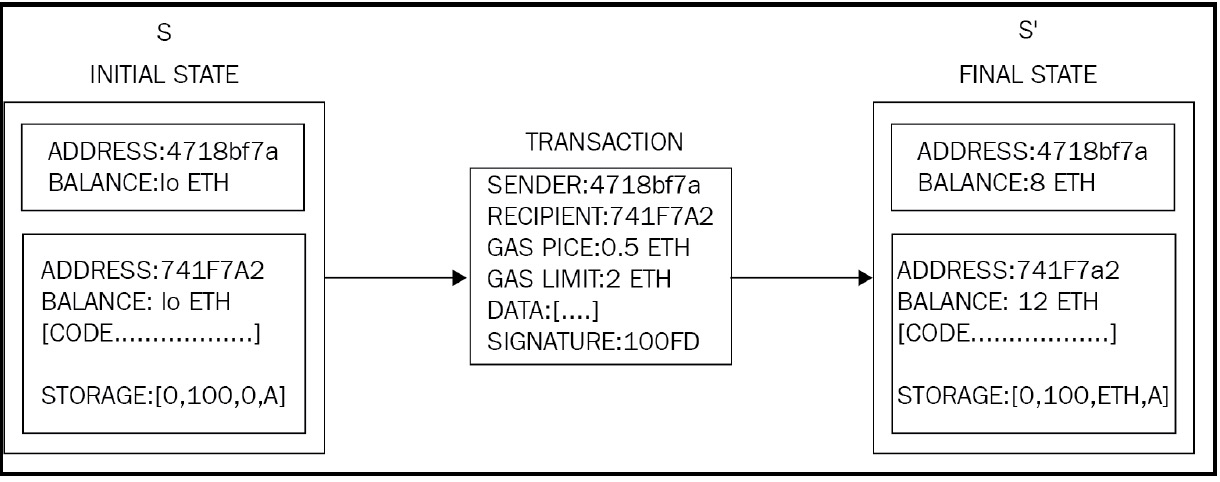
\includegraphics[width=\linewidth]{ethereum_transaction.jpg}
    \caption{Ethereum Transaction \citep{RefWorks:doc:MasteringBlockchain}}
    \label{fig:ethereum_transaction}
\end{figure}

There are currently two Ethereum networks running: Ethereum Classic (ETC) \citep{EthereumClassic} and Ethereum (ETH) \citep{Ethereum}. In this thesis, the Ethereum ETH will be used to discuss and implement the smart contract due to the speculation that the later Ethereum is more popular, advanced and actively maintained. The currency from Ethereum will be refered as "Ether" after this.

\subsection{Smart contract execution on Ethereum}

In Ethereum, each smart contract has its own address after being released to the network. To run one, an user with another Ethereum address will need to initiate a transaction to the contract, which optionally contains the amount of Ether to transfer, the message to invoke some function on the smart contract, and amount of fee (GAS) to be paid for the miners. The transaction will be verified by the network which consumes GAS gradually and if the transaction is invalid, the remaining fee will be refunded to the sender. Otherwise, the amount of Ether specified will be transfer and the code invocation will be activated on the transaction, which will run a specified function on the smart contract.
\chapter{Smart contract development}
\label{ch:smartcontractdev}

Smart contracts are simply programs which run on top of a blockchain network. Hence, they can be developed similarly as normal computer programs, by using programming languages to compile the logic of the software, which then after that being compiled to machine instruction in order to execute. In the Ethereum blockchain, Solidity is introduced to be one of the programming languages which have the support to compile smart contract code \citep{SolidityDocumentation}. 

Solidity is a modern language inspired by many predecessors such as C++, Python and JavaScript \citep{SolidityDocumentation}. It is built with the support for Ethereum Virtual Machine (EVM), which is the platform to execute smart contracts, hence becomes a contract-oriented programming language \citep{SolidityDocumentation}. Together with any other modern counterparts, Solidity features inheritance, statically typed and libraries to ease the development process. To understand later code examples shown in later chapters, the language's features which are contracts, function modifiers, addresses will be described in details

\section{Contracts}

Contracts can be known as the soul of Solidity, and a contract's design reassembles to that of classes in other object-oriented programming languages, with the appearance of state variables equivalent to class properties, functions to class methods. For example, Program \ref{lst:simpleContract} shows a basic contract.

\begin{lstlisting}[float,caption={A simple contract in Solidity.},label={lst:simpleContract},language=Solidity]
pragma solidity ^0.4.0;

contract IntegerStorage {
    uint storedInt; // This is the state variable
    
    function getInt() public returns uint {
        return storedInt;
    }
    
    function setInt(uint newInt) public {
        storedInt = newInt
    }
}
\end{lstlisting}
\label{lst:simpleContract}

Program \ref{lst:simpleContract} shows a contract \texttt{IntegerStorage} which contains a state variable of type \texttt{uint}. This contract also provides two functions, first of which is \texttt{getInt()} which returns the value of the state variable \texttt{storedInt}, and the second is \texttt{setInt(uint newInt)} which receives a parameter of type \texttt{uint} and will set that parameter's value into the state variable

\section{Addresses}

Address is a value type in the Solidity language to denote the Ethereum address, each of which contains a 20-byte value equalling to the size of an Ethereum address \citep{SolidityDocumentation}. The address can be from a real person holding an Ethereum wallet, or another contract, since contracts also own an Ethereum address. This type \texttt{address} includes some members, which is identical to methods and property of an object in other object-oriented programming languages, such as \texttt{balance} and \texttt{transfer}. By having this special value type, it is possible to programmatically send and receive money inside an Ethereum smart contract.

\section{Function modifiers}
\label{section:functionModifiers}

Functions in Solidity contracts can have modifier to change the behavior of its own \citep{SolidityDocumentation}. With function modifiers, methods can be protected by checking a precondition before executing. Program \ref{lst:simpleFunctionModifier} shows a contract which includes a simple function modifier.

\begin{lstlisting}[float,caption={Simple function modifier in a contract \citep{SolidityDocumentation}.},label={lst:simpleFunctionModifier},language=Solidity,float=h,floatplacement=h]
pragma solidity ^0.4.0;

contract OwnedWithModifier {
    function OwnedWithModifier() public { owner = msg.sender; }
    address owner;

    // This contract defines a modifier and it will
    // use it in function close()
    // The function body is inserted where the special symbol
    // `_;` in the definition of a modifier appears.
    // This function modifier ensures that only the
    // owner of this smart contract can execute the close()
    // function and in other cases, an exception will
    // be thrown
    modifier onlyOwner {
        require(
            msg.sender == owner,
            "You need to be the owner to call this function"
        );
        _;
    }
    
    // This function can only execute if the owner
    // is calling it
    function close() public onlyOwner {
        // Do something inside this function
    }
}
\end{lstlisting}

In Program \ref{lst:simpleFunctionModifier}, the contract \texttt{owned} is assigned an Ethereum address coming from the caller of the constructor function, which is included in \texttt{msg} variable, as the owner when being created. During the lifetime of the contract, the function \texttt{close()} can only be effectively executed if the caller's address is equal to the owner's address.

\section{Events}

In order to get the best out of smart contracts, there has to be a method to communicate with them from the applications, website, ... Thus, events are designed as a contract feature in Solidity. Each event contains the data denoted from the time which its contract is created. When being called, the transaction's logs will store the event. Program \ref{lst:contractEvent} and \ref{lst:eventListener} demonstrates a simple interaction from a web application with a smart contract.

\begin{lstlisting}[float,caption={Contract with Event derived from \citep{SolidityDocumentation}.},label={lst:contractEvent},language=Solidity]
pragma solidity ^0.4.0;

contract DepositOrderReceiver {
    event DepositOrderReceiver(
        address indexed _from,
        bytes32 indexed _id,
        uint _value
    );

    function deposit(bytes32 _id) public payable {
        // Events are emitted using `emit`, followed by
        // the name of the event and the arguments
        // (if any) in parentheses. Any such invocation
        // (even deeply nested) can be detected from
        // the JavaScript API by filtering for `Deposit`.
        emit Deposit(msg.sender, _id, msg.value);
    }
}
\end{lstlisting}

\begin{lstlisting}[float,caption={Listening to Event from web applications \citep{SolidityDocumentation}.},label={lst:eventListener},language=JavaScript]
var abi = /* abi as generated by the compiler */;
var DepositOrderReceiver = web3.eth.contract(abi);
var depositReceipt = DepositOrderReceiver.at("0x1234...ab67" /* address */);

// Pass a callback to start watching immediately
var event = depositReceipt.Deposit(function(error, result) {
    if (!error)
        console.log(result);
});
\end{lstlisting}

In Program \ref{lst:contractEvent}, contract \texttt{DepositOrderReceiver} contains a function \texttt{deposit} which emit event \texttt{Deposit} when successfully executed. The event contains the Ethereum address of the sender, the identifier \texttt{\_id} and the amount of deposit \texttt{value}. After being compiled and deployed to the Ethereum network, an identifier called as \texttt{abi} is generated, which can be used from outside of the Ethereum network to specify the contract. In a webpage which embed the JavaScript program \ref{lst:eventListener},  the \texttt{web3} variable is to denote the web3 web framework, which is used to interact with Ethereum network, which then specify to interact with the contract \texttt{DepositOrderReceiver}. The reference to the event \texttt{Deposit} is stored in \texttt{event} variable and then a callback function is passed into which will be invoked everytime the event is emitted.
\chapter{Application Design and Requirements}
\label{ch:ApplicationDesignAndReq}

This chapter will describe the current system of the Blinky mobile application, including the backend server, the clients  and the requirements for the smart contract integration.

\section{System overview and technical terms}

The Blinky mobile application is a cross-platform client written in React Native \citep{ReactNative}, a framework to develop mobile applications using the JavaScript programming language. The usage of the application enables users to register, create a Cost-Split event that happened after he/she paid for one event for everyone and need to split the cost equally and get the part of the money which others owe.

\begin{figure}
    \centering
    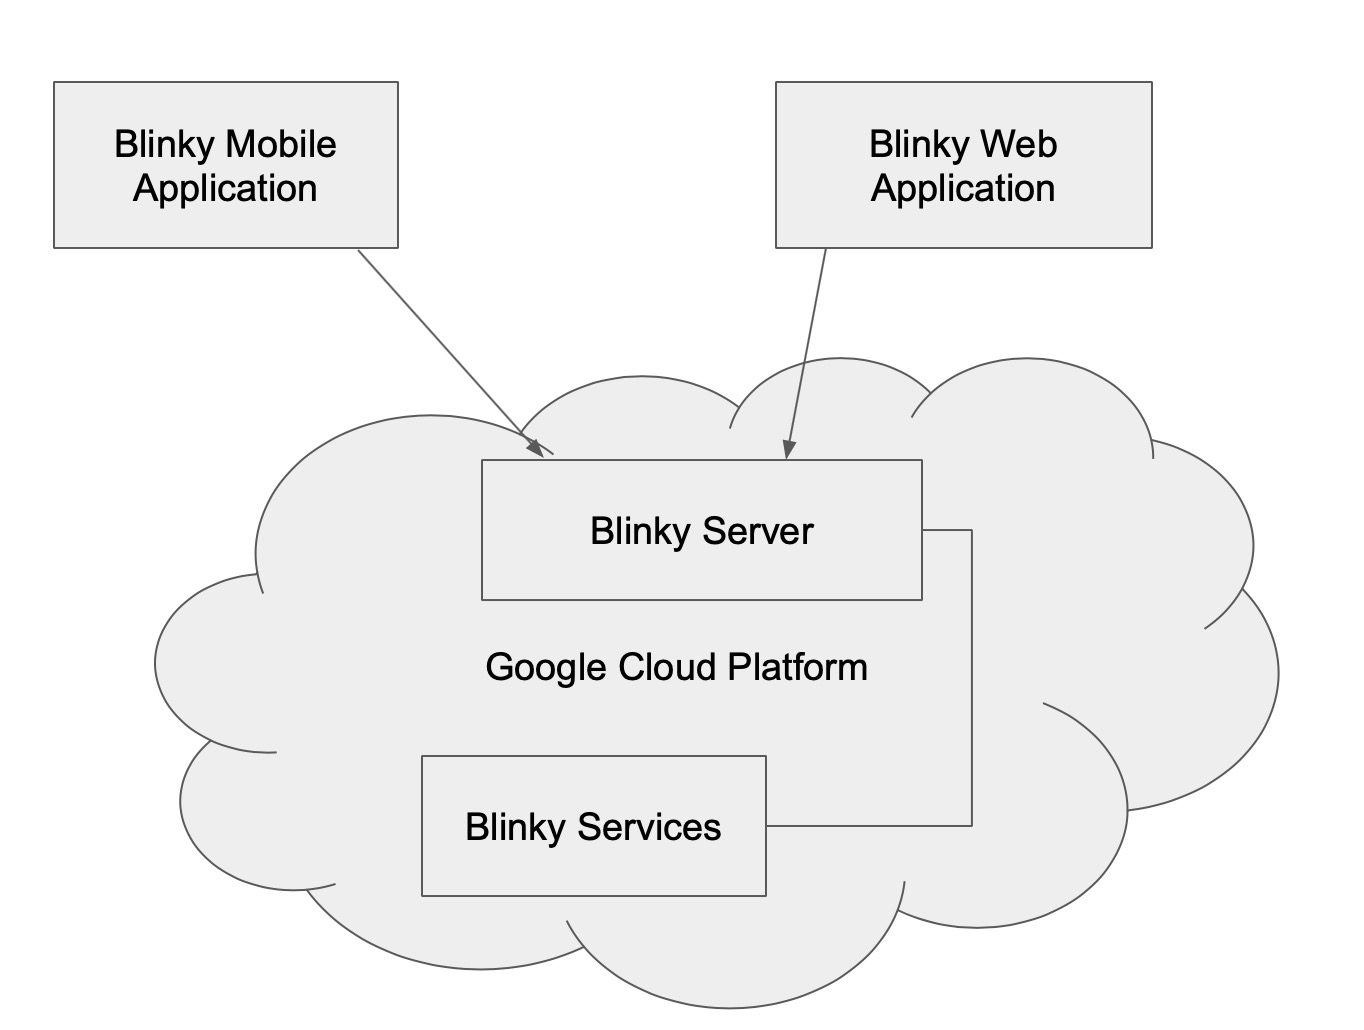
\includegraphics[width=\linewidth]{blinky_system_architecture.jpg}
    \caption{Blinky system architecture}
    \label{fig:blinky_system}
\end{figure}

Users of the Blinky Application can also generate a web URL to share that split cost to friends or relatives. The URL acts as an interface that non-Blinky users can also interact with the services even though they do not have an account. The URL leads to a web application written in React library, which helps building user interface.

Figure \ref{fig:blinky_system} represents the system powering Blinky and where those system are deployed to. 

\section{Application use cases}

The Blinky application was created with the main aim was to help its users to calculate the shares between friends after someone has paid before hand, to ensure a fair and equal split. The application also tries to free users from sticking to one particular payment solution, which allows user to register their preferred payment solution details and later user can share that details together with the calculation details to their friends. Their friends then see the calculation details and take the shared payment method in order to make the payment back to user. From here until the end of this thesis, each of this series of actions from user will be referred as a "Cost-Split" event.

\section{REST API}

The clients, mobile applications and the web application  can communicate with the backend service with a Representational State Transfer (REST)  \citep{REST} Application Programming Interface (API). Data is represented and sent through Javascript Object Notation (JSON).

Users in the mobile application will be granted access right determined by a JSON Web Token (JWT) which can be used in the header of every request to the back-end service. The token contains the user's information which  can easily be used to identify and authenticate them.

The Blinky RestAPI Service will provide an interface for the mobile application so that users can create, edit and delete Cost-Splits, and then invite participants, add expenses to split. Each time a Cost-Split, participant or expense is created on the server, an unique identifier will be generated as an integer and attached to that object. The identifier is then also be used to refer to that object in later actions of its lifetime as well as to delete.
\label{blinkyAPI}

\section{Requirements}
\label{section:requirements}

The requirements for integration with the Ethereum smart contract include:

\begin{itemize}
    \item Generate a new data slot on the smart contract state when a new Cost-Split is created on the application
    \item Increment the data slot with new data each time a Cost-Split is edited with a new user's action such as changing expenses' detail, participants in the Cost-Split, generate an URL, or someone interacted with that URL
\end{itemize}

The requirements are chosen because they depict the common scenarios of transparency between small Cost-Split of a party, such as how much each has to pay, who did declare to have paid.

\subsection{Generating data slot on smart contract}

The desired smart contract will hold a map which contains each Cost-Split's happened event. Each Cost-Split will have its own memory space to store events in a chronological order. Whenever a new event is fired on the client mobile application, a function inside the smart contract should be called provided with the content of the event such as the description, time stamp, user's identifier. The function will then process the input-ed data and append it into that Cost-Split's memory space.

\subsection{Provide a data-retrieval interface for user}

Users of the Blinky application also have the right to request their data in a readable manner, an user-friendly interface. This means that the application will need to provide a function that will represent user and request the data about the user-desired Cost-Split saved on the smart contract. The requested data should also be formatted into a reading-friendly that they can also use as a mean of proof for the action taken by him or anyone interacted with the shared Cost-Split.

\section{Asymptotic Notation}

In order to measure the performance of an algorithm or a computer operation, asymptotic notation is used \citep{AlgorithmAndDataStructure}. In general terms, it is a theoretical framework to measure an algorithm's operation taken to complete the task given a number of inputs. For example, if there is \texttt{n} inputs and the algorithm needs to do \texttt{n} operations on each input, the total number of operations needed to complete the task is \texttt{n * n}, which means it will be exponentially proportional to the number of inputs. In asymptotic notation, only the highest order of operations is taken. From the last example, if the number of operations needed is \texttt{n * n + 2n} then the asymptotic notation is still \texttt{n * n} since it carries order of 2.
\chapter{Implementation}
\label{ch:implementation}

This chapter will describe the proposed solution for implementing a smart contract in this thesis reflecting the requirements outlined in the previous chapter. This will include explaining: 1) The chosen data structure for the smart contract; 2) The necessary functions for the smart contract; 3) Installing the Web3 framework which is used to connect the smart contract to the Blinky application and 4) The solutions to handle potential error during the lifetime of the smart contract.

\section{Smart contract data structure}
\label{section:DataStructure}

In order to write and read Cost-Split data (as described in Section \ref{section:requirements}), the data structure of the smart contract will need to be defined. Figure \ref{fig:smartcontractdatastructure} provides a visualized data structure plan. Since each Cost-Split should have its own space to store its event data, one such option for organizing Cost-Splits could be using a \texttt{mapping} \citep{SolidityMapping}. Each Cost-Split will be identified from the key obtained from the Blinky API server, as described in Section \ref{blinkyAPI}. This will make Cost-Split fetching as quick and efficient because to find an element in a \texttt{mapping} data structure knowing the key (in this case, the Cost-Split's identifier) only need an asymtotic performance of $\Theta(1)$. 

Each event of a Cost-Split will need to carry a description, timestamp and the identifier of the person who initiates the event. Hence, \texttt{struct} data type is the only candidate for defining the data structure of a Cost-Split event. This \texttt{struct} will contain a \texttt{string} type for the description and another \texttt{string} type for the time stamp in the ISO 8601 format \citep{ISOFormat} (such as \texttt{2018-11-12T19:26:47.858Z}) since this format is compatible with various programming languages. The \texttt{struct} will also contain an \texttt{uint} field for storing the user's identifier from Blinky API Service. After this passage, the \texttt{struct} will be refered to as the \texttt{CostSplitEvent} type.
\label{DataStructure}

\begin{figure}[h!]
    \centering
    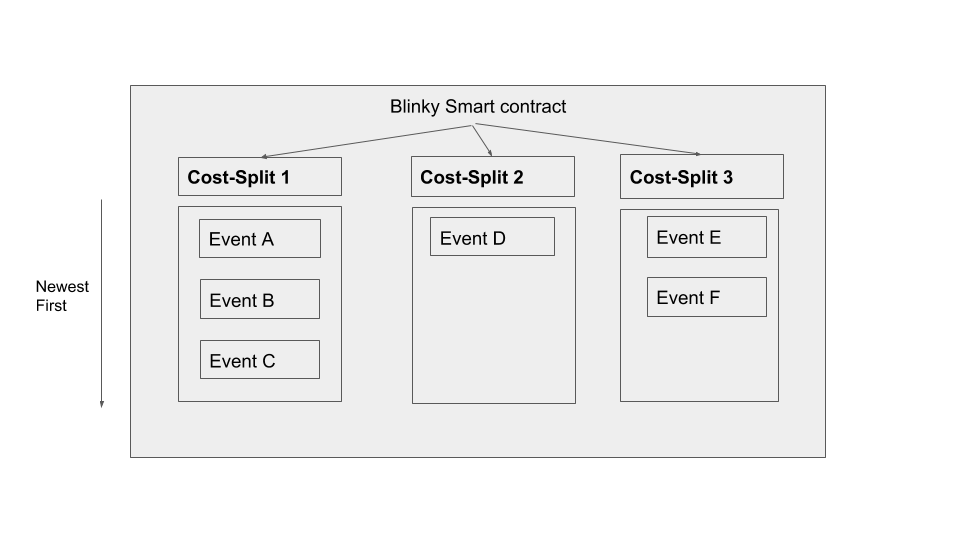
\includegraphics[width=\linewidth]{BlinkyCostSplitSmartContractDataStructure.png}
    \caption{Blinky's Cost-Split Smart contract data structure \citep{RefWorks:doc:MasteringBlockchain}}
    \label{fig:smartcontractdatastructure}
\end{figure}


Furthermore, after being able to access the data of a Cost-Split using its key, each event should be sorted chronologically. Therefore, the smart contract will need to store the Cost-Split data as an \texttt{Array} of \texttt{CostSplitEvent}. Since each event will be recorded chronically by nature, no sorting operation is necessary on the array.

\section{Smart contract functions}
\label{section:SmartContractFunctions}

Since the smart contract will need to be able to create a new data slot for a Cost-Split, a function is needed, which can be named as \texttt{createCostSplit}. This function should accept the identifier of the Cost-Split as a parameter and should return a \texttt{boolean} type to indicate if the creation is successful or not, either \texttt{true} or \texttt{false}.

After a Cost-Split is created, users will then began to interact with it in the Blinky Application, which will incur events. Therefore, a new function is needed to start to add new events into a Cost-Split. This function can be called \texttt{appendEvent}. In order to identify the Cost-Split and to write the necessary data field of the event as specified in Section \ref{DataStructure}, the function will need to receive the identifier of the Cost-Split, the identifier of the Blinky user who initialized the event, the event's time stamp and the event description as the parameter. This function should also denote if the action completes successfully or not so it should return a \texttt{boolean} type like \texttt{createCostSplit}. Figure \ref{lst:appendEventFunction} outlined the function's signature as described above for the purpose of demonstration.

\begin{lstlisting}[float,caption={Skeleton implementation of function \texttt{appendEvent}.},label={lst:appendEventFunction},language=Solidity]

contract BlinkyCostSplit {
 ...
 function appendEvent(
    uint costSplitId,
    uint userId,
    string timestamp,
    string eventDescription) returns (bool) {
   // The function's implementation
   return true;
 }
 ...
}

\end{lstlisting}

In a normal data management software, there should be functions for creating, reading, updating and deleting data. However, in this particular smart contract, data should not be updated or deleted, since the aim of the smart contract is to embrace the transparency, which means data should be as it is from the moment of being created. Users' will to update or delete Cost-Split's events should, therefore, be added to the event list as a new event with the description of what is user's will.

\section{Web3 Framework}

After defining the data structure (mentioned in Section \ref{section:DataStructure}) and the functions needed for the smart contract (as mentioned in \ref{section:SmartContractFunctions} ), knowing a tool for communicating with the smart contract from the outside Internet is necessary, and such an option for it called the Web3 Framework exists. The advantage of this framework that it is written in the Javascript programming language, which is also used in the React Native framework in the Blinky mobile application. Hence, this enables fast and easy integration of the framework to both the web page and the mobile application of Blinky. In order to install and configure the Web3 Framework, the following steps are required:

\begin{itemize}
    \item React Native projects's dependencies can be managed using the \texttt{npm} package manager. Therefore, the content of the Web3 Framework can be downloaded from \texttt{npm}
    \item Choose a suitable Framework version that is compatible with React Native. There are two newest versions: 1.0 and 0.20.x during this time of writing this thesis. Version 1.0's content is generated dynamically, which is not compatible with React Native due to the nature of a mobile application (the code inside the app will be static after being built). Therefore, version 0.22.x is chosen to be installed.
    \item Pony-fill some APIs of Javascript that React Native does not support, such as the \texttt{crypto} API to perform encryption and hashing. Those can be solved by installing package \texttt{node-libs-react-native}
\end{itemize}

There are also community composed tutorials, one of which can be found on the web site link: \citep{InstallWeb3}
After following the above mentioned steps and conducting other smaller tweaks as presented in the link above, The web3 framwework can be invoked in React Native as an example in Program \ref{lst:callweb3}

\begin{lstlisting}[float,caption={Calling Web3 functions and making transactions on the Ethereum blockchain \citep{SolidityDocumentation}.},label={lst:callweb3},language=Javascript]

const web3 = new Web3(Web3.givenProvider);
const contractAddress = "0x1a5c29c94D03C4c8f7414564CBD57295d61e898f";
const contractAbi = [
	{
		"constant": false,
		"inputs": [
			{
				"name": "x",
				"type": "uint256"
			}
		],
		"name": "set",
		"outputs": [],
		"payable": false,
		"stateMutability": "nonpayable",
		"type": "function"
	},
	{
		"constant": true,
		"inputs": [],
		"name": "get",
		"outputs": [
			{
				"name": "",
				"type": "uint256"
			}
		],
		"payable": false,
		"stateMutability": "view",
		"type": "function"
	}
];
const myContract = web3.eth.contract(contractAbi);
myContract.methods.myMethod("set")
  .send({from: '0xde0B295669a9FD93d5F28D9Ec85E40f4cb697BAe'})
  .then(function(receipt){})
  .catch(function (error) {});

\end{lstlisting}

In Program \ref{lst:callweb3}, first an instance of the web3 framework is instantiated, with the default provider bundled within the framework. Then the contract address contract address and it's Application Binary Interface (ABI) is specified in line 3, 4and then passed to the initialization function that creates an instance of \texttt{web3.eth.contract} in line 34, which represents an Ethereum smart contract. After that, the program can start calling the functions on the smart contract by calling function \texttt{methods.myMethod} on the contract instance (as presented in line 36 to 38.

\section{Error handling}

Error handling is one of the most important aspects to consider when developing a software product, to ensure that the software works as expected and maintains a high-quality user experience. In this case of implementing the smart contract for storing Cost-Split event, there are cases which may confuse the smart contract and therefore handling the errors while developing the smart contract is a vital step.

Errors that can happen are when the smart contract tries to add an event to a non-existing Cost-Split, or in other words, the function \texttt{appendEvent} is given an invalid Cost-Split identifier. In solidity, this function invocation will result in throwing an \texttt{Exception}, all the changes to smart contract during that function call will be reverted and the failure will be notified to the caller (in this case, the Blinky Application). However, this kind of error without being handled will degrade user experience since they may not be aware of how the Blinky Application handles the event sending. This thesis will propose a way to handle this error:

 The smart contract's function will use \texttt{require} function as a way to verify the validity of the data (in this case, checking the Cost-Split's identifier if it exists in the smart contract's state). If the assertion does not satisfy, the function will throw an early \texttt{Exception} to tell that the identifier is not valid. The Blinky Application can catch this Exception and display an appropiate dialog to notify user. An example of this error handling is presented in Program \ref{lst:assertValidateInput}. From the Program, it is noted that in Solidity, the default value for a variable is 0 if it has not been set to any value yet. Hence, it is possible to check for the existence of a Cost-Split in the smart contract's state by trying to access its value inside \texttt{mapping costSplitMap}, then compare it to 0. The error message "Cost Split does not exist in the smart contract" will be thrown if the assertion fails.

\begin{lstlisting}[float,caption={Using \texttt{require} function to validate input data},label={lst:assertValidateInput},language=Solidity]
contract BlinkyCostSplit {
 
 struct CostSplitEvent {
    uint userId;
    string description;
    string timestamp
 }
 
 mapping(uint => CostSplitEvent) costSplitMap;
 
 function appendEvent(
    uint costSplitId,
    uint userId,
    string timestamp,
    string eventDescription) returns (bool) {
   // The function's implementation
    require(
        costSplitMap[costSplitId] != 0,
        "Cost Split does not exist in the smart contract"
    );
   // ... Remaining implementation for this function
   return true;
 }
 ...
}
\end{lstlisting}
\chapter{Smart contract evaluation}
\label{ch:evaluation}

This chapter will concentrate on evaluating the smart contract's performance with the mentioned requirement in Chapter \ref{section:requirements}. The evaluation consists of security, privacy, latency and troubleshooting.

\section{Security}
\label{section:security}

Since smart contract is public to the whole blockchain network, there has to be an option to define a rule to execute a function inside a smart contract. Such an option exist in the Solidity language called \textit{function modifier} as mentioned in Section \ref{section:functionModifiers} and a ready-made example in Program \ref{lst:simpleFunctionModifier}. This means the smart contract need to define a modifier that verifies that the function caller is exactly the smart contract owner. To identify who is the owner, the smart contract's constructor need to save the Ethereum address of the caller to one of its own property for later retrieval. This solution provided by Solidity is adequate to protect the smart contract's functions from being called by the unauthorized.

\section{Privacy}

Privacy was not the goal of Ethereum network since every block made in the past can be verified and looked up by the whole network. Therefore, storing the plain data coming from the Blinky application do not provide privacy for user. In order to achieve privacy, the data being sent to smart contract will need to be encrypted. However, a new issue comes up which is who will keep the encryption key. If user is responsible for holding the key, it will require a considerable amount of technical knowledge in order to send and retrieve encrypted data correctly, which will go against the aim of the Blinky application as it tries to provide user the most user-friendly solution. If Blinky application is responsible for holding the encryption key, the aim of decentralized blockchain is also lost since the trust is now given to the Blinky server that it will keep the encryption key secure.

\section{Latency}

The Ethereum network is currently running with the Proof of Work consensus mechanism \citep{RefWorks:doc:BitcoinWhitepaper}, which can only process 15 transactions per second on the whole network, according to the time of writing this thesis. This leads to the unavoided high latency for every time the smart contract is invoked and data is sent. Therefore, interacting with smart contract at this time will not guarantee fast transaction time.
\chapter{Conclusion}
\label{ch:conclusion}

Smart contract can be utilized in social finance application such as the Blinky application which involves in creating and storing event data inside the application. In this work, the Solidity programming language was used to develop a smart contract which acts as a data store for events which happens when user's Cost-Splits incur a new action as mentioned in Sub-Chapter \ref{section:requirements}. The language's documentation is well-written and therefore the smart contract was implemented in a short time interval. Since all the transactions happen inside the Ethereum blockchain and with the necessary security action as mentioned in Sub-Chapter \ref{section:security}, it ensures that the data will maintain its integrity, which will be a basis for a potential legal proof in the future.

By implementing a smart contract and connecting it to the Blinky application, advantages and disadvantages of blockchain can be realized. It is shown that the data state inside the smart contract can be directly requested and appended without going through the Blinky server. This improves the availability and democracy when updating data. Furthermore, it is also shown that the data update to smart contract has to pass the conditions provided in the smart contract's code in order to be accepted. The conditions are verified in every nodes joining the Ethereum network as explained in Sub-Chapter \ref{contentCreationOnBlockchain}. However, as mentioned in Chapter \ref{ch:evaluation}, every transaction or data appending request has to wait for the Ethereum network until it is verified and processed. This is a potential issue that affects user experience since waiting a long time for a small transaction is discouraged. In addition, data on the blockchain does not provide users with privacy (in other words, everyone can request and access data on the blockchain). This also requires users to understand and accept that their data on the blockchain will not be private, unless there are additional encryption methods are applied.

With the advantages and disadvantages of a blockchain-based application, users need to understand what they can take advantage with what drawbacks they have to accept. For some users, this is acceptable. Therefore, it is concluded that this feature of using smart contract in a Blinky's Cost Split should not be used by default. The application should guide user of the feature and its benefits as well as drawbacks.



%\addto\extrasenglish{\btxifchangecaseoff} % Controls the case-changing for English titles. Make sure that case is preserved for abbreviations and proper nouns, e.g. title={The {ABC} of {Tex}: An Introduction to the Typesetting System}

\ifnameyear
  \bibliographystyle{babapaliktutnat}
\else
  \bibliographystyle{bababbrtut}
\fi
\bibliography{references}

\end{document}